\chapter[Boundary layer theory]{Introduction to Boundary Layer Theory (BLT)}
Part VI of the course. Even appears in neurobiology or cardiology. Example, when two different time-scales such as the time for a neuron to charge up (gradual) and then discharge (spike). Boundary layer is when the spike occurs -- matching the slow to fast solutions (could be in time or space). \\
\ \newline
The Boundary Layer theory is a singlular perturbation method that is useful when $\epsilon \ll 1$ multiplies the highest derivative in a differential equation.

\paragraph{Example 1:} Consider
\begin{gather}\label{eqn:wk12-ex1-ode}
	\begin{split}
	\epsilon y'' + (1+\epsilon)y' + y = 0 \\
		y(0)=0 \qquad y(1)=1
	\end{split}
\end{gather}
Let us try the regular perturbation series, meaning we \emph{na\"{i}vely} guess a power series of the form
\begin{gather*}
	y(x,\epsilon) = y_0 + \epsilon y_1(x) + \dots 
\end{gather*}
This yields
\begin{gather*}
	\epsilon (y_0'' + \epsilon y_1'' + \dots) + (1+\epsilon)(y_0' + \epsilon y_1' + \dots ) + (y_0 + \epsilon y_1+\dots ) = 0 \\
	y_0(0) + \epsilon y_1(0) + \dots = 0 + 0\epsilon + \dots \\
	y_0(1) + \epsilon y_1(1) + \dots = 1 + 0\epsilon + \dots
\end{gather*}
resulting in the hierarchy of equations
\begin{align*}
	O(\epsilon^0): \qquad & y_0' + y_0 = 0 \\
	O(\epsilon^1): \qquad & y_0'' + y_0' + y_1' + y_1 = 0
\end{align*}
And this is trouble already! Since we have a first order equation at $O(\epsilon^0)$ yet two BCs (over-determined)! To check explicitly,
\begin{gather*}
	y_0 = c\me^{-x}
\end{gather*}
and since $y_0(0)=0$, it must be that $c=0$. The solution $y_0(x)=0$ does not satisfy the $y_0(1)=1$. Thus the ``regular'' perturbation method fails here and we refer to such problems as ``singular''. \\
\ \newline 
To understand what is going on, we look at the exact solution obtained by trying the soln. form $y = \me^{\lambda x}$:
\begin{gather*}
	\epsilon \lambda^2 + (1+\epsilon) \lambda + 1 = 0
\end{gather*}
This readily yields the roots
\begin{gather*}
	\lambda = -1  \qquad \lambda= -\frac{1}{\epsilon}
\end{gather*}
On application of the two BCs, we arrive at the exact solution
\begin{gather}\label{eqn:wk12-ex1-exact}
	y(x) = \frac{\me^{-x} - \me^{-x/\epsilon}}{\me^{-1} - \me^{-1/\epsilon}}
\end{gather}
Notice the essential singularity $\me^{-x/\epsilon}$. While it appears harmless as it would approach $1/\infty$ as $\epsilon \rightarrow 0^+$, it does not have a convergent Taylor series about $\epsilon = 0$. Therefore the regular perturbative approach, where we can get away with a power series, does not work. 

\paragraph{Explanation:} If we fix $x>0$ and let $\epsilon \rightarrow 0^+$, and say $x\geq 10 \epsilon$ then 
\begin{gather}\label{eqn:wk12-ex1-approx}
	y(x) \rightarrow \me^{1-x}
\end{gather}
If $x\sim \epsilon$ then the $\me^{-x/\epsilon}$ term cannot be ignored. From Fig. \ref{fig:strogatz-wk12} it is evident that as $x$ gets smaller, $\epsilon$ must decrease to get a closer match with the asymptotic expression. This is point-wise convergence and not uniform convergence. For any $\epsilon$, the match is quite good in the region $x \geq 10\epsilon$.
\begin{figure}[!h]
	\centering
	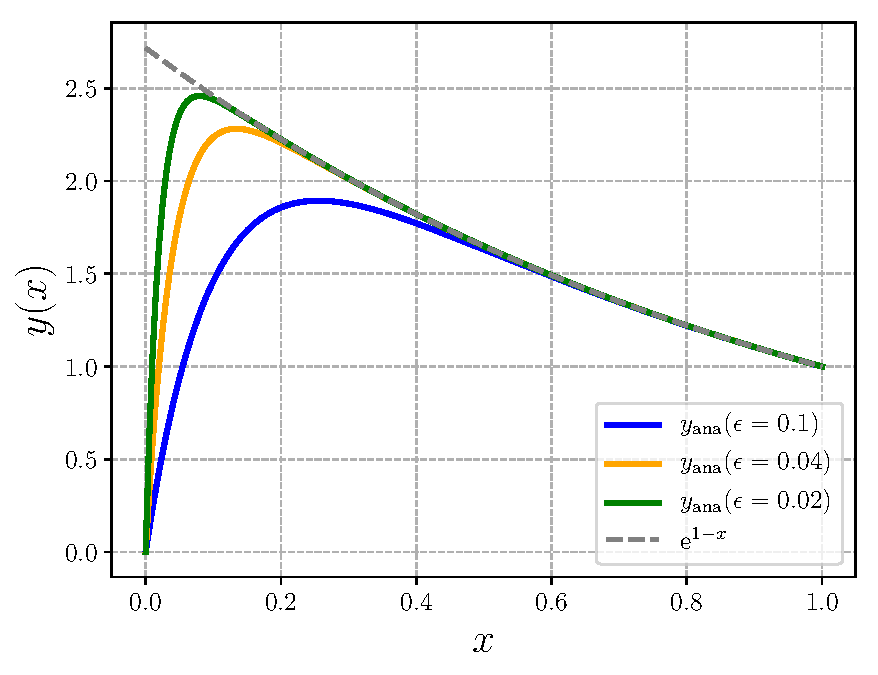
\includegraphics[width=0.65\textwidth]{./plots/pdf/strogatz-wk12.pdf}
	\caption{Plotting the exact soln. \ref{eqn:wk12-ex1-exact} and the asymptotic soln. \ref{eqn:wk12-ex1-approx}.}
	\label{fig:strogatz-wk12}
\end{figure} \\
The region of rapid change near $x=0$ (namely $0<x<O(\epsilon)$) is called a ``boundary layer''. The boundary layer is the ``inner'' region and the region away from it is called the ``outer'' region. 

\paragraph{Solution:} Using a technique called ``matched asymptotic expansions''. First attempt the \underline{outer region} solution using regular perturbation theory: we think of $x$ as fixed and let $\epsilon \rightarrow 0^+$ and solve the ODE with the right BC at $x=1$. So we solve
\begin{gather*}
	y_0' + y_0 = 0 \qquad y_0(1) = 1
\end{gather*}
yielding
\begin{gather}
	y_0(x)_\mathrm{out} = \me^{1-x}
\end{gather}
Going to the $O(\epsilon)$ problem
\begin{align*}
	y_1' + y_1 &= -y_0' - y_0'' \\
		&= -(\underbrace{y_0 + y_0'}_0)'
\end{align*}
which with the appropriate BC at $x=1$ yields
\begin{gather*}
	y_1(x) = 0
\end{gather*}
For this problem $y_2 = y_3 = \dots = 0$. \\
\ \newline
Now we look at the \underline{inner region}. We introduce a new `stretched' variable $X = x/\epsilon$, since this is the natural length-scale defined in the question. In our $X$ scale, the BL is at $X \rightarrow \infty$. Our transformed ODE reads
\begin{gather}\label{eqn:wk12-inner-ode}
	\frac{\md^2 Y}{\md X^2} + (1+\epsilon) \frac{\md Y}{\md X} + \epsilon Y = 0
\end{gather}
Observe that when $\epsilon = 0$, we do not loose the highest derivative! In some sense, the rapid variation through $Y_{XX}$ multiples with the $\epsilon$ term to be finite and not zero. We now use regular perturbation theory on this re-scaled inner ODE. The BC is now 
\begin{gather*}
	y(0) = 0 \qquad Y(X=0) = 0 + 0\epsilon + \dots 
\end{gather*} 
Let
\begin{gather*}
	Y_\mathrm{inn} = Y_0 + \epsilon Y_1 + \dots 
\end{gather*}
which yields 
\begin{gather*}
	(Y_0'' + \epsilon Y_1'' + \dots ) + (1+\epsilon)(Y_0' + \epsilon Y_1' + \dots ) + \epsilon(Y_0 + \epsilon Y_1 + \dots) = 0
\end{gather*}
and the ordered set of equations
\begin{align*}
	O(\epsilon^0): \qquad & Y_0'' + Y_0' = 0 \\
	O(\epsilon^1): \qquad & Y_1'' + Y_1' + Y_0' + Y_0 = 0
\end{align*}
The $O(\epsilon^0)$ equation is solved by one trivial integration and then solving the resultant first order ODE with the integrating factor method. This yields
\begin{gather*}
	Y_0 = A + B\me^{-X}
\end{gather*}
With the BC imposed we derive
\begin{gather*}
	Y_0(X) = A (1 - \me^{-X})
\end{gather*}
where the parameter $A$ is what would help match the inner and outer solutions.

\paragraph{Overlap region \& composite expansion:} The condition on the matching region is
\begin{align*}
	\lim\limits_{X \rightarrow \infty} Y_0(X) &= \lim\limits_{x\rightarrow 0} y(x)_\mathrm{out} \\
	A &= \me
\end{align*}
{\bf NB:} We have effectively done a zeroth order matching! In some problems we may need to match solutions at higher orders too. That said, zeroth order matching is usually sufficient in practice. The uniformly valid \emph{composite} approximation is expressed as
\begin{align*}
	y_c &= y_\mathrm{out} + Y_\mathrm{inn} - y_\mathrm{match} \\
	&= \me^{1-x} + \me (1-\me^{x/\epsilon}) - \me \\
	&= \me (\me^{-x} - \me^{-x/\epsilon})
\end{align*}
which is related to our exact solution eqn. \ref{eqn:wk12-ex1-exact} as
\begin{gather*}
	y(x) = \frac{y_c}{1 - \me^{1-1/\epsilon}}
\end{gather*}
For a moderately low $\epsilon=0.1$, the denominator is $1 - \me^{-9} \approx 1 - 10^{-4} \approx 1$. 
\begin{figure}[!h]
	\centering
	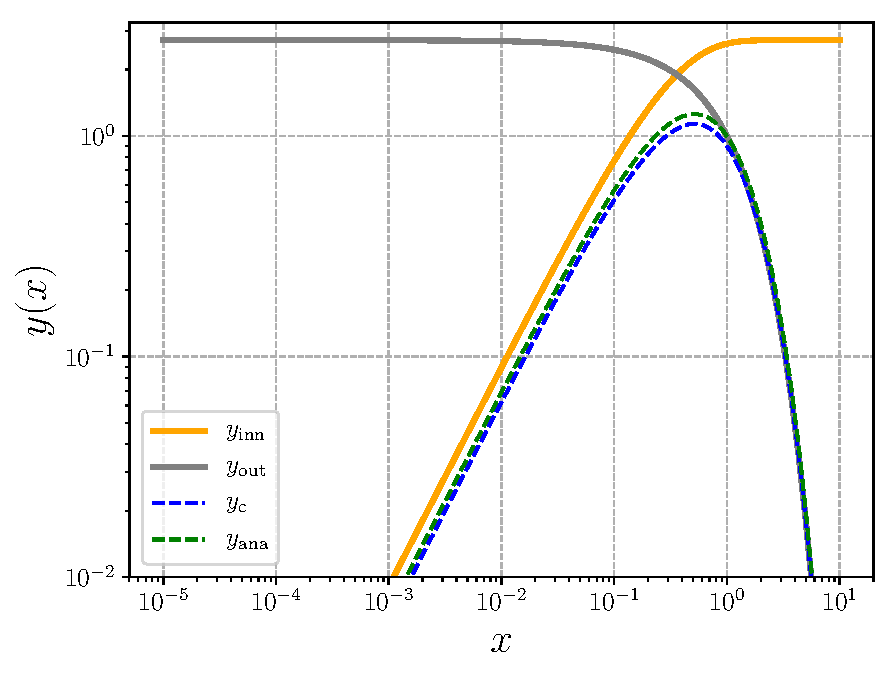
\includegraphics[width=0.75\textwidth]{./plots/pdf/strogatz-wk12-composite-eps3e-1.pdf}
	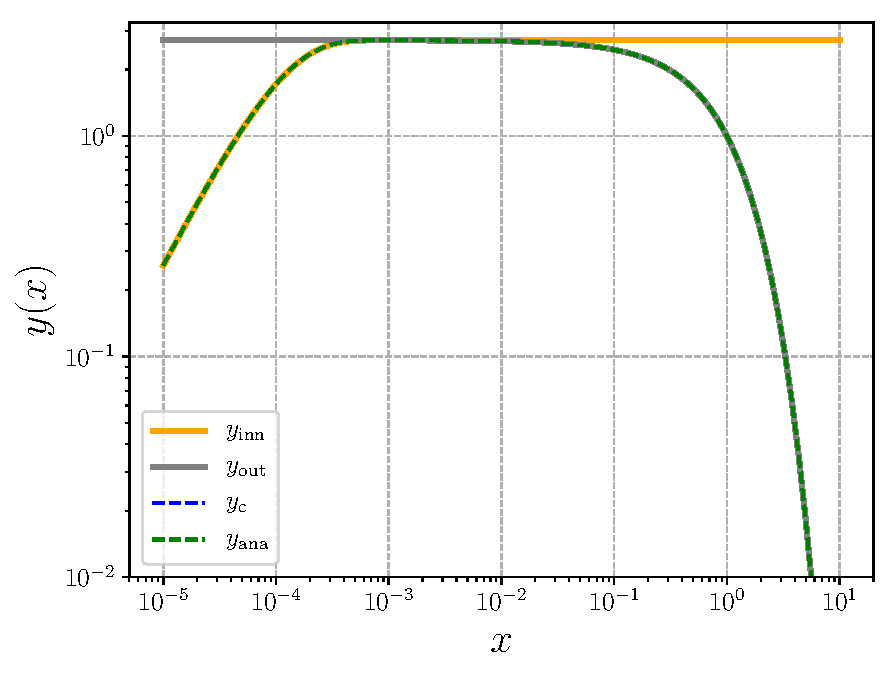
\includegraphics[width=0.75\textwidth]{./plots/pdf/strogatz-wk12-composite-eps1e-4.pdf}
	\caption{The various solution forms plotted for (top) $\epsilon = 0.3$ and (bot) $\epsilon=10^{-4}$.}
	\label{fig:strogatz-wk12-composite}
\end{figure} 
\begin{itemize}
	\item Note that the overlap region ceases to exist as $\epsilon$ is increased. {\bf Why?}
\end{itemize}